PathCase and its related tools exist in a rich ecosystem of databases, display
methods, graph algorithms, and input methods. The iPathCase tools are intended
to unify this ecosystem as much as possible.

\section{Databases}

Existing pathway data sources include KEGG, BioCyc, and Reactome. The Kyoto
Encyclopedia of Genes and Genomes (KEGG) is the primary database resource of the
Japanese GenomeNet service for understanding higher order functional meanings
and utilities of the cell or the organism from its genome information
\cite{kegg-basic}. This database was discussed in section
\ref{sect:background_kegg}.

The KEGG web site visualizes pathways using static images like the one shown in
figure \ref{fig:kegg_site_viz}.

\begin{figure}[hbtp]
    \center{
        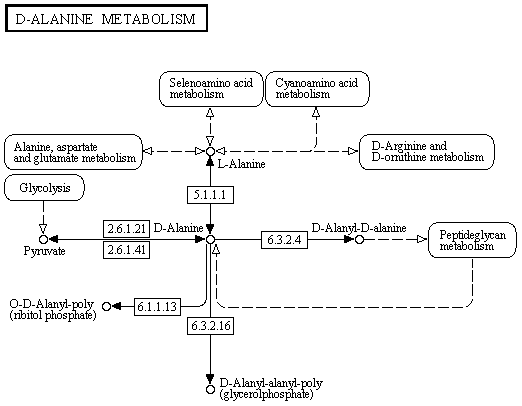
\includegraphics[width=4in]{fig/kegg_d-alanine_metabolism}}
    \caption{\label{fig:kegg_site_viz} KEGG visualization of D-Alanine
    metabolism}
\end{figure}

The BioCyc collection of Pathway/Genome Databases (PGDBs) provides an electronic
reference source on the genomes and metabolic pathways of sequenced organisms
\cite{biocyc}. The level of curation of the PGDBs ranges from intensive to
nonexistent, and they are categorized as such.

The BioCyc web site visualizes pathways using static images like the one shown
in figure \ref{fig:biocyc_site_viz}.

\begin{figure}[hbtp]
    \center{
        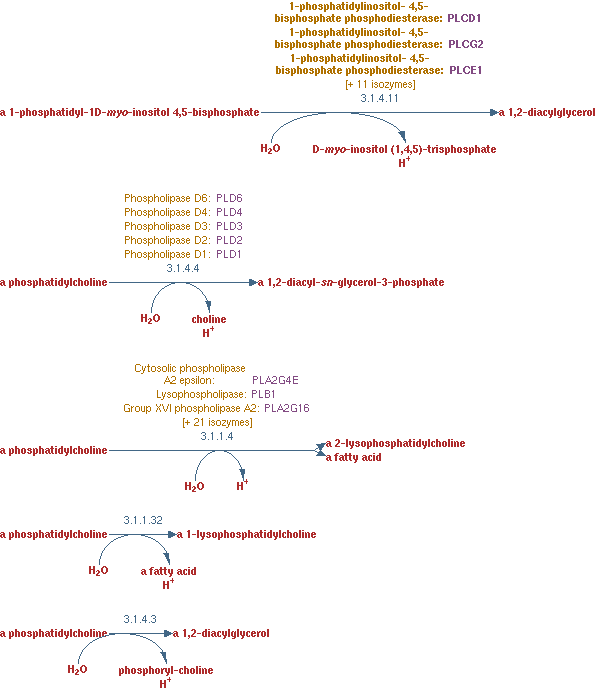
\includegraphics[width=4in]{fig/biocyc_phospholipases}}
    \caption{\label{fig:biocyc_site_viz} BioCyc visualization of phospholipases}
\end{figure}

Reactome is an open-source, open access, manually curated and peer-reviewed
pathway database \cite{reactome}. Pathway annotations are authored by expert
biologists, in collaboration with Reactome editorial staff and cross-referenced
to many bioinformatics databases.

The iPathCase tools do not use any of these databases directly, but may access
them through PathCase in the future. \keggapp does provide links to these
databases for pathways and enzymes where appropriate, but does not otherwise
make use of them.

\section{Input Methods}

The iPathCase tools combine the simplicity of the online PathCase tools with the
tactile input methods of the iPad.

\begin{figure}[hbtp]
    \center{
        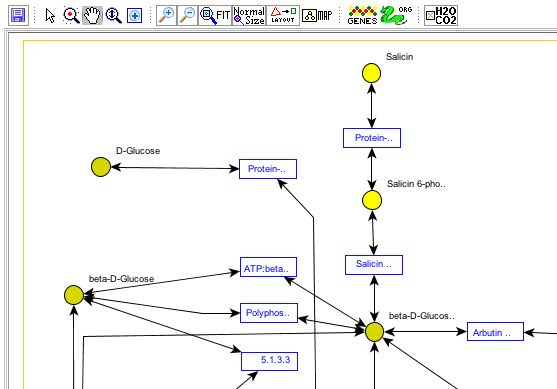
\includegraphics[width=4in]{fig/pathcase_kegg_online_viz}}
    \caption{\label{fig:pathcase_kegg_online_viz} PathCase KEGG online
    visualization of glycolysis}
\end{figure}

The online PathCase KEGG visualizer, shown in figure
\ref{fig:pathcase_kegg_onine_viz}, presents a graph of the pathway which can be
panned and zoomed using modal mouse-based tools. Nodes can be moved by clicking
and dragging. The iPathCase visualizers are based on the same principles but
make use of modeless multitouch gestures instead of modal tools selected on a
toolbar. Many of these gestures are identified by Frisch et al
\cite{multitouch:gestures} and the iOS Application Programming Guide
\cite{ios:application-programming-guide}.
